\section{Internals}\label{sec:internal}
\subsubsection{What are ``service contracts''?}\label{sec:internal:contracts}
\emph{Service contracts}, as implemented by the acs-service-contract
package of the OpenACS core, introduces \emph{call abstraction}, a
concept with as many dimensions as actual areas of usage, to OpenACS
as framework. The idea is not to reproduce existing documentation on
service contracts, but to generalise the problem tackled by
contracts. Service contracts aim at providing some sort of
re-usability and a generic extension mechanism at the framework
level. Call abstraction is a generic concept that can be found at the
level of programming languages (of various flavours, OO and non-OO,
functional etc.) and as infrastructure facilities in frameworks of
various kind. The general motivation for call abstraction is a
twofold: First, we want to assemble complex code blocks (i.e. a proc,
involving sequences of calls to other code blocks) at design time
(i.e. the time we conceptualise and write our program). Second,
however, we do not want to specify a concrete addressee of some calls
in our code block at run time. Call abstraction might be referred to
as \emph{identity transparency} which simply means the actual
addressees or callees are not determined at design time! The simple
motivation for these two requirements is that we want to allow varying
behaviour within a more generally designed picture. Varying behaviour
should be able to be introduced in a pre-defined and standardised
manner. Let's take an example, taken from the OO-verse of XOTcl which
gives a nice show case example, easier graspable than a general
description of service contracts as such.
%
\lstset{breaklines=true,numbers=left,basicstyle=\footnotesize,frame=single}
\lstinputlisting[firstnumber=1,firstline=4,lastline=13]{../examples/xorb/example-01-call-abstraction.xotcl}
%
Imagine, you set out to provide an full-text search in your
application. In OpenACS, you might think of the "search" package as a
direct example. An important role in this infrastructure module is
played by an indexer that either on-demand or at regular intervals
triggers the indexation of new text items. The indexer is represented
by an XOTcl object "Indexer" that offers a method "index" responsible
for the actual indexing walk-through. The fundamental design problem
now is how to provide for the possibility to add new kinds of
indexable items at an arbitrary point in time after the design and
implementation of the indexer as such. To make it short, how to
provide extensibility to the indexer? Key to an appropriate solution
is the definition of a generic interface which needs to implemented by
all indexable items that might be added in the future.
%
\lstinputlisting[firstnumber=last,firstline=15,lastline=16]{../examples/xorb/example-01-call-abstraction.xotcl}
%
This "caller interface", represented by the XOTcl class "Indexable"
shown above, stipulates an abstract call "getContent" that needs to be
resolved to a concrete call at runtime. Resolving means, in an OO
setting, that implementing sub-classes of Indexable come with a
non-abstract method "getContent". At \begin{math}t_0\end{math},
i.e. design and implementation time of the infrastructure module, the
per-object method "index" therefore exclusively refers to an abstract
call "getContent". This is also known as template method, a prominent
design pattern documented by \cite{gof:1994}.
%
\lstinputlisting[firstnumber=last,firstline=18,lastline=26]{../examples/xorb/example-01-call-abstraction.xotcl}
%
As can be seen from the above snippet, by implementing "Indexable" and
providing a concrete method "getContent" forum entries will be indexed
upon future runs of the indexer, i.e. calls to "index". Registration,
in our example, is realised by establishing a sub class relationship
to Indexable. If, at \begin{math}t_1\end{math}, wiki pages should be
also be included in the full-text index, another specialised sub class
of Indexable is needed:
%
\lstinputlisting[firstnumber=last,firstline=37,lastline=44]{../examples/xorb/example-01-call-abstraction.xotcl}
%
This is a simple sketch of what extensibility is in this
reading. Note, call abstractions in various settings come with
different connotations (i.e. semantics), but they share basic
ideas. Coming back to "service contracts" that realise call
abstractions at a non-OO framework level, you might think of "service
contracts" as abstract classes such as Indexable in the above example
and of "service implementations" as registrars, represented by
creating a sub class of Indexable. A more generic picture of call
abstraction is given by Figure \ref{fig:advanced:ca:1}:
  \begin{figure}[htbp]
\begin{center}
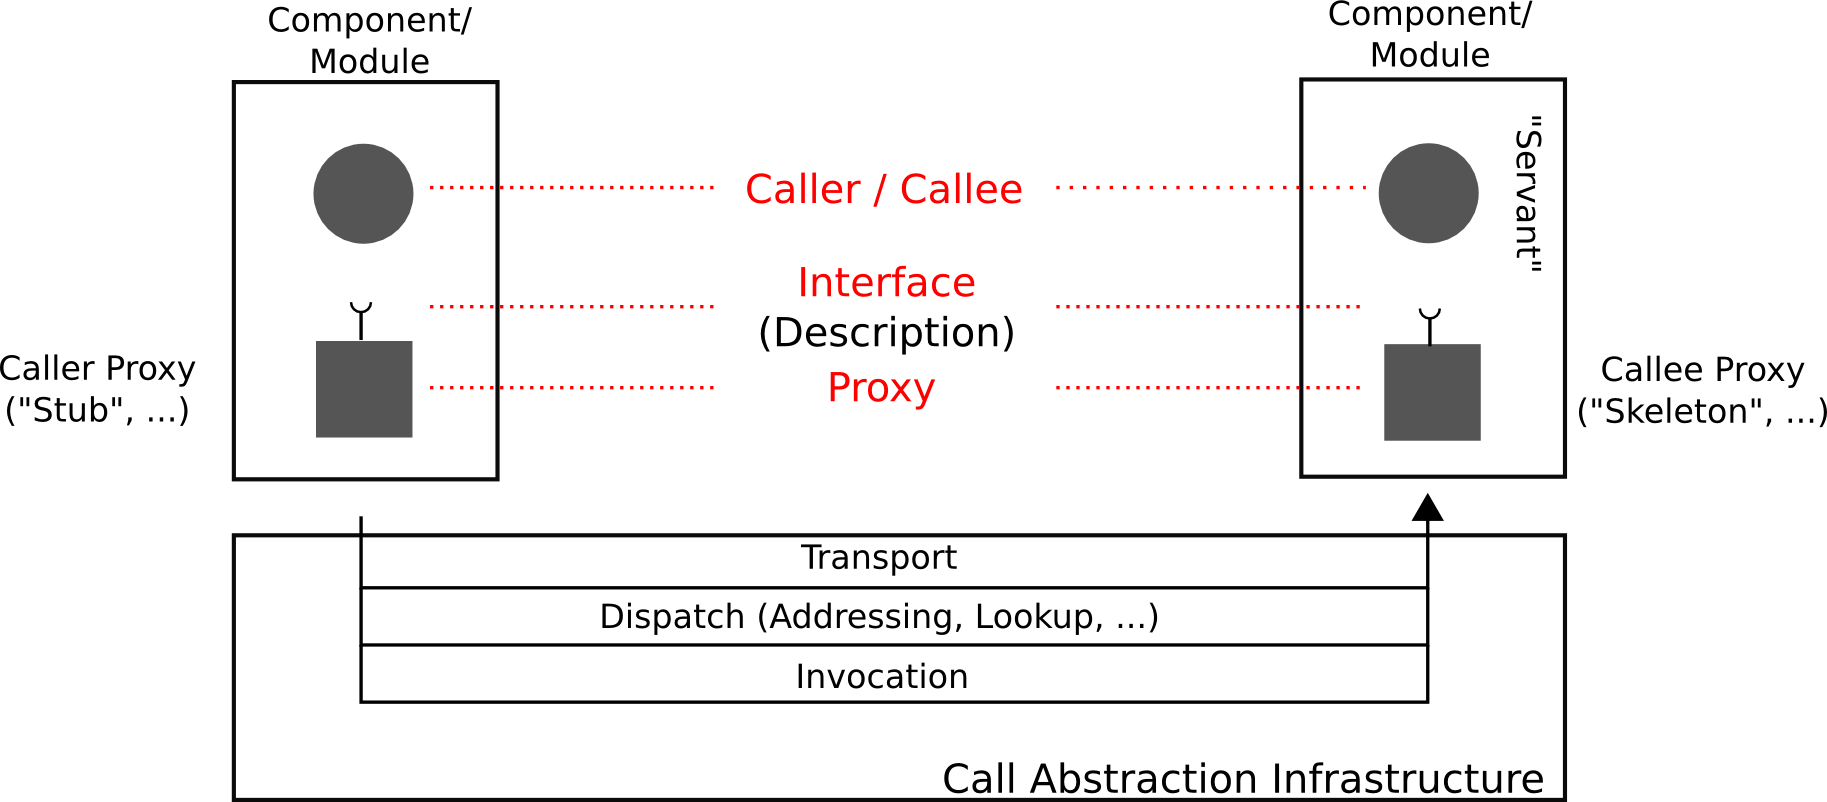
\includegraphics[width=0.55\textwidth]{img/call-abstraction-scheme.png}
\caption{Call abstraction}
\label{fig:advanced:ca:1}
\end{center}
\end{figure} The XOTcl example (and OpenACS service contracts) would
translate into the following roles shown by the schematic outline: The
class Indexable (a service contract such as FtsContentProvider)
stipulates takes the role of \emph{interface (descriptions)}. In this
role, they have two responsibilites, first interfacing to the caller
(caller interface) and interfacing to the callee (callee
interface). The caller is an arbitrary code block that issues the
index call on objects of type Indexable. The callee, or servant, is
the concrete getContent method of any sub class derived from class
Indexable (e.g. XowikiPage, or, the service implementation
content\_revision). The proxy role is taken by the getContent method
defined on Indexable and declared abstract (in OACS service contracts,
these are operations defined on contracts).

A final clarification is needed at this point: What has become known
as "remote procedure calls" (RPC) or "remote method invocations" (RMI)
is the basic idea of call abstraction, but identity transparency is
accompanied by \emph{location transparency}.